\section{Einleitung}

In dieser Ausarbeitung soll eine Methode beschrieben werden, mit deren Hilfe man durch endlich viele Zufallszahlen 
eine ungefähr gleichmäßige Verteilung von Punkten im Raum generieren kann. Damit kann man sehr gut Daten simulieren, 
welche eine bestimmte Verteilung besitzen und, wie in der Natur üblich, keine harten Kanten besitzen oder komplett 
zufällig verteilt sind, sondern abfallen. Zu diesen Dichteverteilungen gehört zum Beispiel auch die Gaußschen Normalverteilung. 

Für die randomisierten Eingaben werden sogenannte "Golden Ratio Sequences", die von Schretter 
\cite{schretter-golden_ratio_sequences-2012} vorgestellt wurden, verwendet. Diese Punkte werden auf die von Chen 
und Asau \cite{chen_asau-generating_random_variates-1974} und Devroye \cite{devroye-non_uniform_random_variate-1986} 
beschriebene, verbesserte \hyperref[funktion]{Inversionsmethode} mit Hashing angewandt, wodurch das gewünschte Ergebnis 
erzielt wird. Diese Verfahrenskette wird unter \hyperref[impl]{Implementation} näher erläutert und durchgeführt. 


\subsection{Problemstellung}
Durch diese Ausarbeitung soll geklärt werden, wie die Hash-basierte Inversionsmethode funktioniert und ob  
sie bei der Generierung von multivariaten Verteilungen in höheren Dimensionen mithilfe von uniformen Dichten immer noch 
korrekt arbeitet und einsetzbar ist. Außerdem soll verglichen werden, ob sich der Einsatz der hier beschriebenen 
Methode als Ersatz von bereits existierenden anderen Methoden lohnt.

\begin{figure}
    \centering
    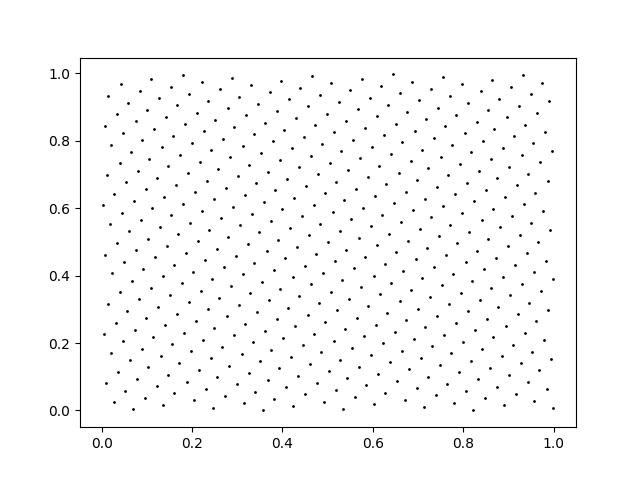
\includegraphics[width=0.48\textwidth]{grs_u500c.png}
    \caption{500 gleichmäßige, zufällige Punkte einer Goldenen-Schnitt-Sequenz \cite{schretter-golden_ratio_sequences-2012}.}
\end{figure}

\subsection{Stand der Technik}
Anstelle der hash-basierten Inversionsmethode kann auch ein Feld der Partialsummen der einzelnen Wahrscheinlichkeiten 
der zu generierenden Punkte verwendet werden. Auf dem Feld können dann unterschiedliche Methoden zum Finden der Werte 
verwendet werden. Dazu gehören lineare Suche von vorne nach hinten, binäre Suche oder ein Huffman-Baum.

Zur Generierung uniformer Zufallszahlen gibt es anstelle der Sequenzen des goldenen Schnittes auch Methoden wie
die von Halton \cite{wong_luk_heng-halton_points_sampling-1997}, Blue Noise \cite{yan-blue_noise_sampling-2015} oder Rang-1-Gitter 
\cite{prasad-rank1lattice-1973}. Doch da Schretter in seinem Paper zeigt, dass die von diesen Methoden generierten Zahlen 
nicht so gleichmäßig verteilt generiert werden, wie seine Vorgestellte \cite{schretter-golden_ratio_sequences-2012}, 
wird jene verwendet. 